\section{Experiment 1 - How boundaries affect advection with semi Lagrangian time integration}
In this experiment we would like to examine how the boundaries affect our advection. In this week's notebook we have worked with the peaks functions, and used advection with semi Lagrangian time integration to turn the scalar field 360 degrees around. This can be seen in \autoref{original} and we will use this as a baseline comparison for our experiment.
\begin{figure}[H]
	\centering
	\begin{subfigure}[b]{0.40\linewidth}
		\centering
		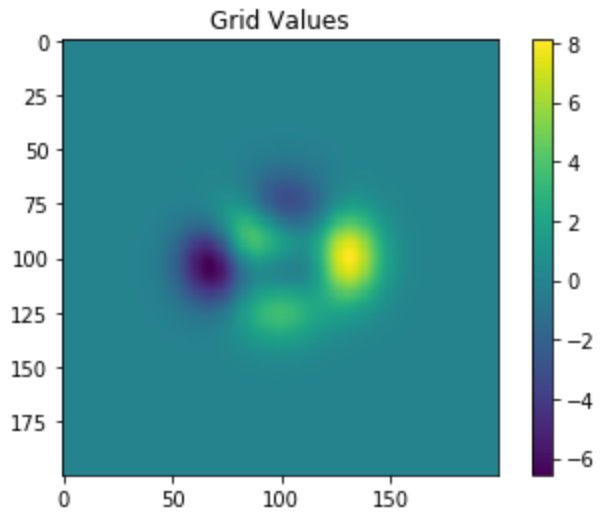
\includegraphics[width=\linewidth]{Materials/Lagrangian/ot0}
		\caption{Image of peaks function before advection.}
		\label{ot0}
	\end{subfigure}
	\hfill
	\begin{subfigure}[b]{0.40\linewidth}
		\centering
		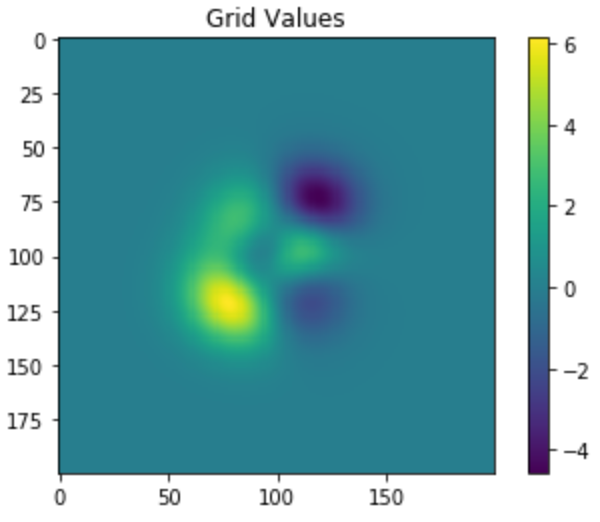
\includegraphics[width=\linewidth]{Materials/Lagrangian/ot1}
		\caption{Image of peaks function after $\frac{1}{2}\pi$ rotation.}
		\label{ot1}
	\end{subfigure}
	\\
	\begin{subfigure}[b]{0.40\linewidth}
		\centering
		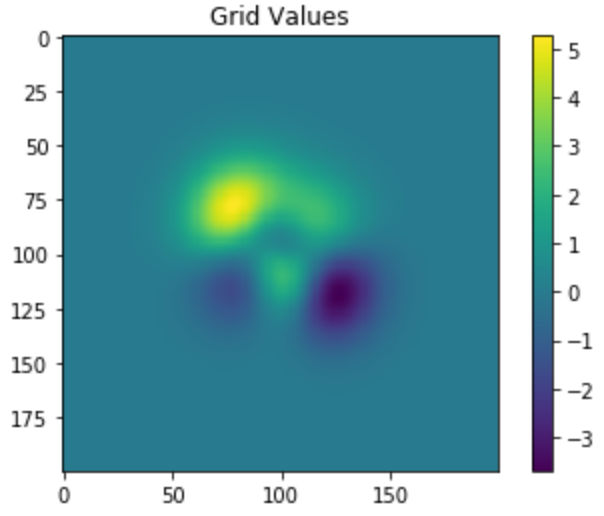
\includegraphics[width=\linewidth]{Materials/Lagrangian/ot2}
		\caption{Image of peaks function after $1\frac{1}{1}\pi$ rotation.}
		\label{ot2}
	\end{subfigure}
	\hfill
	\begin{subfigure}[b]{0.40\linewidth}
		\centering
		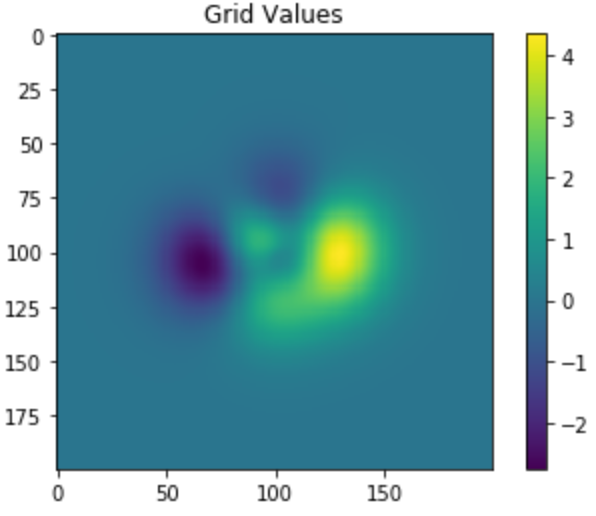
\includegraphics[width=\linewidth]{Materials/Lagrangian/ot3}
		\caption{Image of peaks function after $2\pi$ rotation.}
		\label{ot3}
	\end{subfigure}
	\caption{Advection without any boundary issues. The grid is defined over the domain $-5$ to $5$ with 200 grid nodes along each axis, and with $\Delta t = 0.0005$.}
	\label{original}
\end{figure}
As we see this is no perfection advection, and we have an error of $0.21$, meaning we loose about $21\%$ mass. We also note we are not having any issues with boundaries, as the peaks rotate in the middle of the grid without hitting the boundaries. We can now shrink the grid such that when rotating the peaks we will move outside the grid. The previous grid was defined over the domain $-5$ to $5$, we now shrink this to $-1.5$ to $1.5$.
\begin{figure}
	\centering
	\begin{subfigure}[b]{0.40\linewidth}
		\centering
		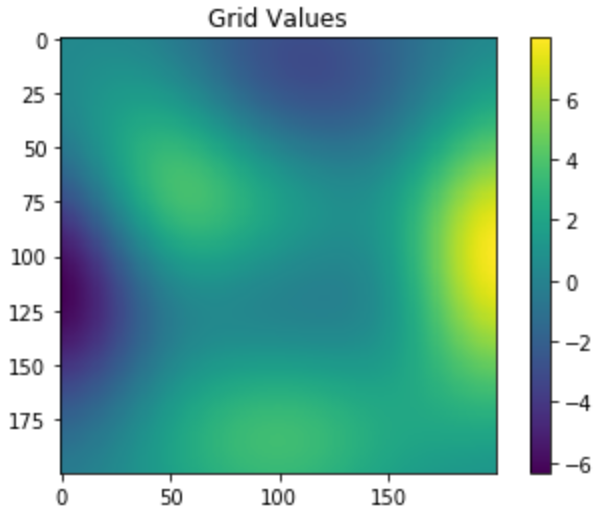
\includegraphics[width=\linewidth]{Materials/Lagrangian/et0}
		\caption{Image of peaks function before advection.}
		\label{et0}
	\end{subfigure}
	\hfill
	\begin{subfigure}[b]{0.40\linewidth}
		\centering
		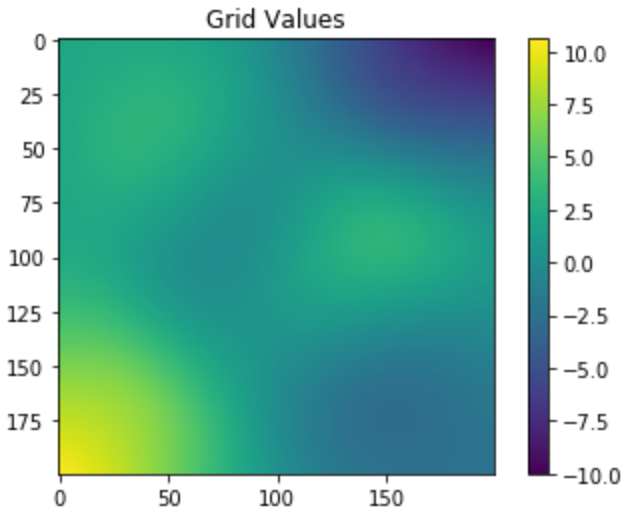
\includegraphics[width=\linewidth]{Materials/Lagrangian/et1}
		\caption{Image of peaks function after $\frac{1}{2}\pi$ rotation.}
		\label{et1}
	\end{subfigure}
	\\
	\begin{subfigure}[b]{0.40\linewidth}
		\centering
		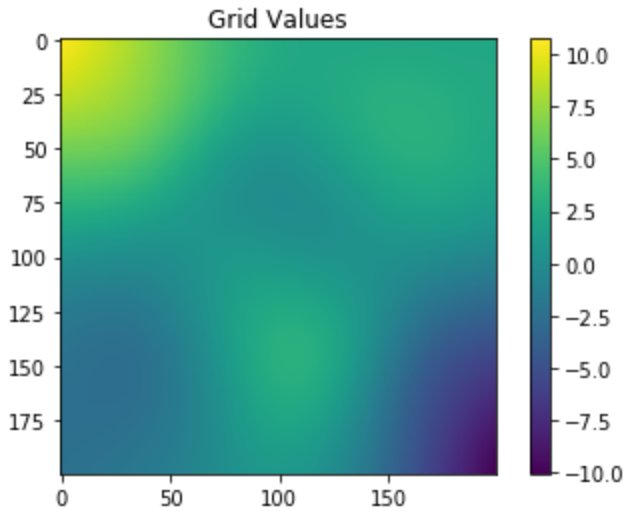
\includegraphics[width=\linewidth]{Materials/Lagrangian/et2}
		\caption{Image of peaks function after $1\frac{1}{1}\pi$ rotation.}
		\label{et2}
	\end{subfigure}
	\hfill
	\begin{subfigure}[b]{0.40\linewidth}
		\centering
		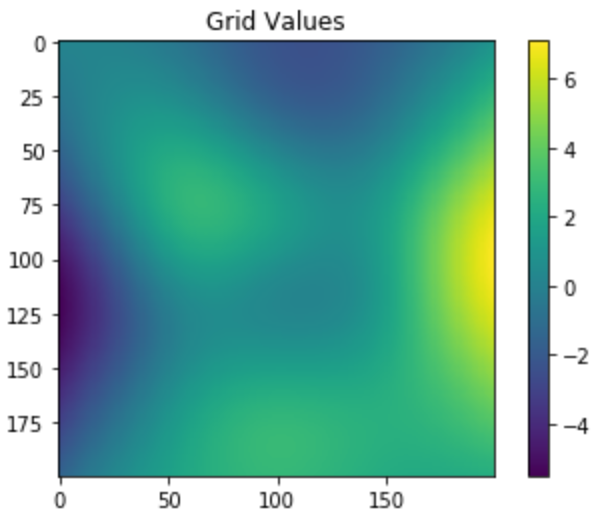
\includegraphics[width=\linewidth]{Materials/Lagrangian/et3}
		\caption{Image of peaks function after $2\pi$ rotation.}
		\label{et3}
	\end{subfigure}
	\caption{Advection with boundary issues. The grid is defined over the domain $-1.5$ to $1.5$ with 200 grid nodes along each axis, and with $\Delta t = 0.0005$.}
	\label{experiment1}
\end{figure}
In \autoref{experiment1} we see the results of shrinking the grid. When comparing \autoref{ot0} and \autoref{et0} we do not see too much of a difference except we have 'zoomed in'. However, comparing \autoref{ot1} with \autoref{et1} and \autoref{ot2} with \autoref{et2} we see that the 'shapes' are similar, but that the peaks have become a lot larger in the corners of \autoref{et1} and \autoref{et2} and similarly the big canyon have becomes much deeper. This is to the extend that the smaller peaks in the experiment images have grown almost as large as the original large peak. We also see that the small canyon in the lower right corner of \autoref{et1} and lower left corner of \autoref{et2} have been somewhat leveled out. When comparing \autoref{ot3} and \autoref{et3} we see pretty much the same shapes but we again see the scaling of the peaks have changed, although not as drastically as for the intermediate rotations.

\subsection{Discussion of results}
We see when we shrink the domain that instead of the peaks and canyons going towards 0 they actually become bigger. As they rotate, they move outside our grid, and thus we need to interpolate them back in. In this process we compute the new grid value based on an interpolation to the nearest grid cell. The fact we move outside the grid causes us to lose information about the peaks and canyons and because we use the neighbourhood around the nearest grid cell we also a slight error in the computed value as it actually should have been computed at a slightly different location. These are probably the causes we see a different behaviour of the peaks and canyons compared to when we do not have any boundary issues. The interpolation used to get the results for this experiment is the interpolation function in this week's notebook.
